\begin{example}
    \textbf{Меры.}
    \begin{enumerate}
        \item Классический объём $\lambda_m$ (потом докажем)
        \item $g: \R \rightarrow \R$ неубывающая, непрерывная справа во всех точках
        
        $\nu_g(a, b]:=g(b) - g(a)$

        \begin{exercise}
            Доказать, что непрерывность справа – необходимое условие для того,
            чтобы $\nu_g$ была мерой.
        \end{exercise}

        \item $x_0\in X$, $a>0$, $\mu A=\left\{\begin{array}{ll}
            a, & \text{если } x_0\in A \\
            0, & \text{иначе}
        \end{array}\right.$
        \item Считающая мера $\mu A=$ количество элементов в множестве $A$.
        \item $T=\{t_1, t_2, ...\}\subset X$, $\{w_1, w_2, ...\}$ –  неотрицательные числа, $\mu A:=\sum\limits_{i:t_i\in A}w_i$

        \begin{proof}
            Нужно проверить, что если $A=\bigsqcup\limits_{j=1}^\infty A_j$, то $\mu A = \sum \limits_{j=1}^\infty\mu  A_j$. 
            
            $\mu  A_j=\sum \limits_{k=1}^\infty a_{jk}$, $\mu A = \sum a_{jk}$ в каком-то порядке $\underset{}{\overset{?}{=}}\sum \limits_{j=1}^\infty \sum \limits_{k=1}^\infty a_{jk}$

            $\geq$: $\underset{\overset{n\rightarrow \infty}{\rightarrow} \sum \limits_{j=1}^\infty\sum \limits_{k=1}^\infty a_{jk}}{\sum \limits_{j=1}^n\sum \limits_{k=1}^\infty a_{jk}}=\sum \limits_{k=1}^\infty\sum \limits_{j=1}^n a_{jk} \leq \mu A$

            $\leq$: Расcмотрим частичную сумму для $\overset{\rightarrow \mu A}{\sum a_{jk}}$. $Y := \max j$, $K := \max k$.

            $\sum \limits_{j=1}^\infty\sum \limits_{k=1}^\infty a_{jk}\geq \sum \limits_{j=1}^Y\sum \limits_{k=1}^\infty a_{jk}\geq \sum \limits_{j=1}^Y\sum \limits_{k=1}^K a_{jk}$

        \end{proof}
    \end{enumerate}
\end{example}

\begin{theorem}
    Пусть $\mu: \mathcal{P} \rightarrow [0, +\infty]$ – объем на полукольце. 
    
    Тогда $\mu $ – мера $\Leftrightarrow$ (счетная полуаддитивность) Если $P, P_n\in \mathcal{P}, P \subset\bigcup\limits_{n=1}^\infty P_n$, 
    то $\mu P \leq \sum\limits_{n=1}^\infty \mu P_n$.
\end{theorem}

\begin{proof}~
    \begin{enumerate}
        \item[$\Leftarrow$.] Если $P=\bigsqcup\limits_{n=1}^\infty P_n$
            \begin{enumerate}
                \item счетная полуаддитивность $\Rightarrow \mu P \leq \sum\limits_{n=1}^\infty \mu P_n$
                \item усиленная монотонность $\Rightarrow \mu P \geq \sum\limits_{n=1}^\infty \mu P_n$
            \end{enumerate}
        \item[$\Rightarrow$.] $P_n':= P \cap P_n \in \mathcal{P} \Rightarrow P = \bigcup\limits_{n=1}^\infty P'_n\Rightarrow 
        P = \bigsqcup\limits_{n=1}^\infty\bigsqcup\limits_{k=1}^{m_k}Q_{nk}$, где $Q_{nk}\in \mathcal{P}$, $Q_{nk} \subset P'_n \subset P_n$

        $\mu P = \sum\limits_{k=1}^\infty \sum\limits_{k=1}^{m_k} \mu Q_{nk} \leq \sum \limits_{n=1}^\infty \mu P_n$

        $\bigsqcup\limits_{k=1}^{m_k} Q_{nk}\subset P_n\overset{\text{усил. монот.}}{\Rightarrow}\sum\limits_{k=1}^{m_k}\mu Q_{nk}\leq \mu P_n$
    \end{enumerate}
\end{proof}

\begin{corollary}
     Если $\mu$ – мера, заданная на $\sigma$-алгебре, то счетное объединение
     множеств нулевой меры – множество нулевой меры.
\end{corollary}

\begin{proof}
    $\mu _n = 0$, $A=\bigsqcup\limits_{n=1}^\infty A_n\overset{\text{счет. полуад.}}{\Rightarrow} \mu A_n \leq \sum\limits_{n=1}^\infty \mu A_n=0\Rightarrow \mu A=0$
\end{proof}

\begin{theorem}
    Пусть $\mu$ – объем, заданный на $\sigma$-алгебре $\mathcal{A}$. 
    
    Тогда $\mu$ – мера $\Leftrightarrow$ (непрерывность снизу) Если $A_1 \subset A_2 \subset ....$, $A_n\in \mathcal{A}$,
    то $\mu (\bigcup\limits_{n=1}^\infty A_n) =\lim \mu A_n$.
\end{theorem}

\begin{proof}~
    \begin{enumerate}
        \item[$\Rightarrow$.] $B_k := A_k \setminus A_{k-1}$ (считаем, что $A_0=\varnothing$)
        
        $A:=\bigcup\limits_{n=1}^\infty A_n \underset{\supset}{=} \bigsqcup\limits_{n=1}^\infty B_n$ ($B_n \subset A_n$)

        $\subset$: если $x\in A$, то возьмем $m$ – наименьший индекс, для которого $x\in A_m\Rightarrow x\in B_m$.

        (счет. ад.) $\mu A= \sum \limits_{n=1}^\infty \mu B_n = \sum \limits_{n=1}^\infty(\mu A_n - \mu A_{n-1})$

        Если все $\mu A_n$ конечны, то $\underset{\rightarrow \sum \limits_{k=1}^\infty \mu B_k=\mu A}{\sum \limits_{k=1}^n \mu B_k} = \sum \limits_{k=1}^n (\mu A_k - \mu A_{k-1})=\mu A_n\Rightarrow \mu A_n\rightarrow \mu A$

        Если $\mu A_n=+\infty$ при больших $n$, то $\mu A=+\infty$ и все очевидно.

        \item[$\Leftarrow$.] Пусть $A=\bigsqcup \limits_{n=1}^\infty C_n$, $A_n:=\bigsqcup \limits_{k=1}^n C_k$, $A_1\subset A_2 \subset ...$ и $\bigcup\limits_{n=1}^\infty A_n = A$
        
        $\overset{\text{непр. снизу}}{\Rightarrow}\underset{=\mu (\bigsqcup\limits_{k=1}^n C_k)=\sum\limits_{k=1}^n\mu C_k}{\mu A_n}\rightarrow \mu A
        \Rightarrow \mu A = \sum\limits_{k=1}^\infty \mu C_k$
    \end{enumerate}
\end{proof}

\begin{theorem}
    Пусть $\mu$ –  объем, заданный на $\sigma$-алгебре $\mathcal{A}$ и $\mu X< +\infty$, 
    тогда следующие условия равносильны:
    \begin{enumerate}
        \item $\mu$ – мера.
        \item $\mu$ непрерывно сверху, т.е. если $A_1 \supset A_2 \supset ...$ и $\bigcap\limits_{n=1}^\infty A_n = :A$, 
        то $\mu A_n \rightarrow \mu A$.
        \item $\mu$ непрерывна сверху на пустом множестве, т.е. если $A_1 \supset A_2 \supset ...$ и $\bigcap\limits_{n=1}^\infty A_n = \varnothing$, то $\mu A_n \rightarrow 0$.
    \end{enumerate}
\end{theorem}

\begin{proof}~
    \begin{enumerate}
        \item[$2. \Rightarrow 3.$] Очевидно.
        \item[$1. \Rightarrow 2.$] $B_n := A_1 \setminus A_n$,   $B_1 \subset B_2 \subset B_3 \subset ...$
        
        $\bigcup\limits_{n=1}^\infty B_n = \bigcup\limits_{n=1}^\infty (A_1 \setminus A_n) = A_1 \setminus \bigcap\limits_{n=1}^\infty A_n = A_1 \setminus A\Rightarrow
        \underset{=\mu(A_1\setminus A_n)=\mu A_1 - \mu A_n}{\mu B_n} \rightarrow \mu (A_1\setminus A) = \mu A_1-\mu A$

        \item[$3. \Rightarrow 1.$] Пусть $A=\bigsqcup\limits_{n=1}^\infty C_n$, $A_n:=\bigsqcup\limits_{k=n+1}^\infty C_k$, $A_1 \supset A_2 \supset ...$ 
        
        $\bigcap\limits_{n=1}^\infty A_n =\varnothing$, $A=A_n \sqcup \bigsqcup\limits_{k=1}^n C_k\overset{\mu\text{ – объем}}{\Rightarrow}
        \mu A = \underset{\rightarrow 0}{\mu A_n}+\underset{\rightarrow\sum\limits_{k=1}^\infty \mu C_k}{\sum\limits_{k=1}^n \mu C_k}\Rightarrow
        \mu A = \sum\limits_{k=1}^\infty \mu C_k$
    \end{enumerate}
\end{proof}

\begin{corollary}
    Если $A_1 \supset A_2 \supset ...$ и $\mu A_n < +\infty$ для некоторого
    $n$, то $\mu A_k \rightarrow \mu (\bigcap\limits_{n=1}^\infty A_n)$.
\end{corollary}

\begin{remark}
    Конечность меры существенна.

    $A_n = [n, +\infty)$, $\mu A_n = +\infty$, $\bigcap\limits_{n=1}^\infty A_n =\varnothing$.
\end{remark}

\subsection{Продолжение меры}

\begin{definition}
    $\nu: 2^X \rightarrow [0, +\infty)$ – \textit{субмера}, если:
    \begin{enumerate}
        \item $\nu \varnothing =0$
        \item $A\subset B\Rightarrow \nu A\leq \nu B$ (монотонность)
        \item $\nu(\bigcup\limits_{n=1}^\infty A_n)\leq \sum\limits_{n=1}^\infty \nu A_n$ (счетная полуаддитивность)
    \end{enumerate}
\end{definition}

\begin{definition}
    $\mu: \mathcal{A}\rightarrow [0, +\infty)$ – \textit{полная мера}, если $A\subset B \in \mathcal{A}$ и $\mu B=0$, 
    то $A\in \mathcal{A}$.
\end{definition}

\begin{remark}
    Если $\mu$ – полная мера, $A\subset B$ и $\mu B = 0$, то $\mu A = 0$.
\end{remark}

\begin{definition}
    Пусть $\nu$ – субмера. Множество $E$ назовем \textit{измеримым относительно $\nu$}, если $\forall A\subset X$, $\nu A = \nu (A\cap E) + \nu (A\setminus E)$.
\end{definition}

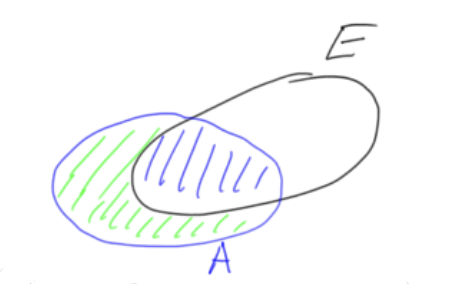
\includegraphics[width=0.2\linewidth]{images/23-09-14-1.png}

\begin{remark}~
    \begin{enumerate}
        \item Достаточно писать «$\leq$», т.к. счетная полуаддитивность $\Rightarrow $
        
        $\nu (A\cap E) + \nu (A\setminus E)\geq \nu \underset{=A}{((A\cap E) \cup (A\setminus E))}$.
        \item Если $E_1, E_2, ..., E_n$ – $\nu$-измеримые, то $\nu \underbrace{(A\cap \bigsqcup\limits_{k=1}^n E_k)}_{\bigsqcup\limits_{k=1}^n(A\cap E_k)=:B}=\sum\limits_{k=1}^n \nu (A\cap E_k)$

        $\nu B = \nu (\underset{=A\cap E_1}{B\cap E_1})+ \nu (\underset{=\bigsqcup\limits_{k=2}^n(A\cap E_k)}{B\setminus E_1})$
    \end{enumerate}
\end{remark}

\begin{theorem}
    \textbf{Теорема Каратеодори}

    Пусть $\nu$ – субмера. Тогда $\nu$-измеримые множества образуют $\sigma$-алгебру и сужение $\nu$ на эту 
    $\sigma$-алгебру – полная мера.
\end{theorem}

\begin{proof}~
    $\mathcal{A}$ – семейство $\nu$-измеримых множеств $E$

    \begin{enumerate}
        \item Если $\nu E=0$, то $E\in \mathcal{A}$.
        
        $\nu A \overset{\text{полуад.}}{\leq} \nu \overset{\subset A}{(A\cap E)}+\nu \overset{\subset E}{(A\setminus E)}\overset{\text{монот.}}{\leq} \nu E + \nu A = \nu A$

        \item $\mathcal{A}$ – симметрично.
        
        Пусть $E\in \mathcal{A}\Rightarrow \nu A = \nu (\underset{=A\setminus(X\setminus E)}{A\cap E})+\nu (\underset{=A\cap(X\setminus E)}{A\setminus E})=
        \nu (A\setminus(X\setminus E))+\nu (A\cap(X\setminus E))\Rightarrow X\setminus E\in \mathcal{A}$

        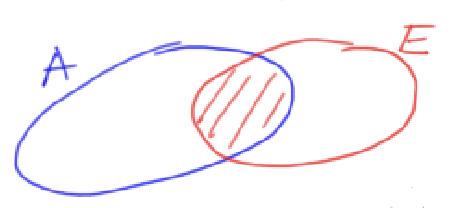
\includegraphics[width=0.2\linewidth]{images/23-09-14-2.png}

        \item Если $E$ и $F\in \mathcal{A}$, то $E\cap F \in \mathcal{A}$
        
        $\nu A = \nu (A\cap E)+\nu (A\setminus E)= \nu (A\cap E)+\nu ((A\setminus E)\cap F)+\nu (\overset{=A\setminus (E\cup F)}{(A\setminus E)\setminus F})\overset{\text{счет. полуад.}}{\geq} 
        \nu (A\cap(E\cup F))+\nu (A\setminus (E\cup F))$

        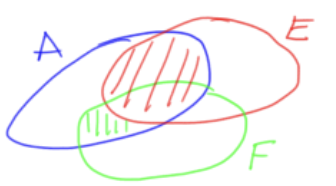
\includegraphics[width=0.2\linewidth]{images/23-09-14-3.png}

        \item $\mathcal{A}$ – алгебра.
        \item Если $E_n\in \mathcal{A}$, то $\overset{=:E}{\bigsqcup\limits_{n=1}^\infty E_n}\in \mathcal{A}$.
        
        $\nu A=\nu (A\cap \bigsqcup\limits_{k=1}^n E_k)+\nu (A\setminus \bigsqcup\limits_{k=1}^n E_k)=
        \sum \limits_{k=1}^n \nu(A\cap E_k) + \nu (A\setminus E_k)\geq
        \sum \limits_{k=1}^n \nu(A\cap E_k) + \nu (A\setminus E)\rightarrow
        \sum \limits_{k=1}^\infty \nu(A\cap E_k) + \nu (A\setminus E)\overset{\text{счет. полуад.}}{\geq} \nu (A\cap E) + \nu (A\setminus E)$

        \item Если $E_n\in \mathcal{A}$, то $\bigcup\limits_{n=1}^\infty E_n\in \mathcal{A}$.
        
        Переделаем в дизъюнктное объединение.

        \item $\mathcal{A}$ – $\sigma$-алгебра.
        
        Из 4 и 5.
        \item $\nu$ – объем.
        
        $\nu(\bigsqcup\limits_{k=1}^n (A\cap E_k))=\sum\limits_{k=1}^n \nu(A\cap E_k)$

        Если $A$ –  любое и $E_k\in \mathcal{A}$, берем $A=X$ и получаем определение объема.

        \item Объем + счетная полуаддитивность $\Rightarrow$ мера.
    \end{enumerate}
\end{proof}

\begin{definition}
    Пусть $\mu$ – мера на полукольце $\mathcal{P}$. \textit{Внешней мерой}, порожденной $\mu$, назовем
    $\mu^* A:=\inf \{\sum\limits_{k=1}^\infty \mu A_k\mid A_k\in \mathcal{P}\text{ и } A\subset \bigcup\limits_{k=1}^\infty A_k\}$.

    Если такого покрытия не существует, то $\mu^* A = +\infty$.
\end{definition}

\begin{remark}~
    \begin{enumerate}
        \item Можем рассматривать только дизъюнктные множества:
        
        $\bigcup\limits_{k=1}^\infty A_k = \bigsqcup\limits_{n=1}^\infty\bigsqcup \limits_{k=1}^{m_k} B_k$, 
        $B_k\in \mathcal{P}$ и $\bigsqcup\limits_{k=1}^{m_k} B_k \subset A_k\overset{\text{усил. монот.}}{\Rightarrow}\mu A_k \geq \sum \limits_{k=1}^{m_k} \mu B_k$

        \item Если $\mu$ задана на $\sigma$-алгебре $\mathcal{A}$, то:
        
        $\mu^*A :=\inf \{\mu B\mid A \subset B\text{ и } B \in \mathcal{A}\}$
    \end{enumerate}
\end{remark}

\begin{theorem}
    $\mu^*$ – субмера, совпадающая с $\mu$ на $\mathcal{P}$.
\end{theorem}

\begin{proof}~
    \begin{enumerate}
        \item Пусть $A\in\mathcal{P}$. Тогда можно взять такие покрытия: $A_1=A$, $A_2=A_3=...=\varnothing\Rightarrow \mu^* A\leq \mu A$
        
        Счетная полуаддитивность $\Rightarrow$ если $A\subset \bigcup\limits_{n=1}^\infty A_n$, 
        то $\mu A \leq \sum \limits_{n=1}^\infty \mu A_n\Rightarrow \mu A \leq \mu^* A$

        т.е. $\mu^* =\mu$ на $\mathcal{P}$

        \item $\mu^*$ – субмера 
        
        \textit{Монотонность:} 
        
        Если есть $A\subset B$ и покрытие $B\subset \bigcup\limits_{n=1}^\infty B_n$, то $A\subset \bigcup\limits_{n=1}^\infty B_n\Rightarrow
        \underset{\inf \text{ от большего мн-ва}}{\mu^* A} \leq \mu^*B$ 
        
        \textit{Счетная полуаддитивность $\mu^*$:} 
        
        $\mu^*$: $\mu^*(\bigcup\limits_{n=1}^\infty B_n)\leq \sum\limits_{n=1}^\infty \mu^* B_n$ 
        
        Если справа есть $+\infty$, то очевидно, считаем, что там все конечно:

        $\mu^* B =\inf \{\sum\limits_{k=1}^\infty \mu P_k\mid P_k\in \mathcal{P}\text{ и } B_n\subset \bigcup\limits_{k=1}^\infty P_k\}$

        Выберем такие множества $C_{nk}$, что $\bigcup\limits_{k=1}^\infty C_{nk}\supset B_n$ и $\sum\limits_{k=1}^\infty \mu C_{nk}\leq \mu^* B_n +\frac{\varepsilon}{2^n}$

        $\bigcup\limits_{n=1}^\infty B_n\subset \bigcup\limits_{n=1}^\infty\bigcup\limits_{k=1}^\infty C_{nk}\Rightarrow 
        \mu^* (\bigcup\limits_{n=1}^\infty B_n)\leq \sum\limits_{n=1}^\infty\sum\limits_{k=1}^\infty \mu C_{nk}\leq
        \sum\limits_{n=1}^\infty (\mu^* B_n + \frac{\varepsilon}{2^n})=\sum\limits_{n=1}^\infty \mu^* B_n + \varepsilon$ и устремим $\varepsilon$ к нулю.
    \end{enumerate}
\end{proof}

\begin{definition}
    \textit{Стандартное продолжение меры $\mu_0$ с полукольца $\mathcal{P}$}.

    Берем $\mu_0^*$ – ее внешняя мера и $\mu$ – сужение $\mu_0^*$ на $\mu_0^*$-измеримые множества. 
    Получается полная мера, заданная на $\sigma$-алгебре.
\end{definition}

\begin{theorem}
    Это действительно продолжение, то есть множества из $\mathcal{P}$ будут $\mu$-измеримыми.
\end{theorem}

\begin{proof}
    Надо доказать, что если $E\in \mathcal{P}$, то $\forall A\subset X$ $\mu_0^* A \geq \mu_0^* (A\cap E)+\mu_0^* (A\setminus E)$

    \begin{enumerate}
        \item Если $A\in \mathcal{P}$, то $A\setminus E =\bigsqcup \limits_{k=1}^n Q_k$, где $Q_k\in \mathcal{P}$. 
        Тогда т.к. $A=(A\cap E)\sqcup \bigsqcup \limits_{k=1}^n Q_k$:

        $\mu_0^* A = \mu_0 A \overset{\text{адд.}}{=}\mu_0(A\cap E)+\sum \limits_{k=1}^n \mu_0 Q_k=\mu^*_0(A\cap E)+\sum \limits_{k=1}^n \mu^*_0 Q_k
        \overset{\text{полуадд.}}{\geq} \mu_0^* (A\cap E)+\mu_0^* (\bigsqcup \limits_{k=1}^n Q_k)= \mu_0^* (A\cap E)+\mu_0^* (A\setminus E)$

        \item Если $A\not\in \mathcal{P}$. Когда $\mu_0^* A=+\infty$ все очевидно, поэтому будем считать, что $\mu_0^* A<+\infty$.
        
        $\mu^* A:=\inf \{\sum\limits_{k=1}^\infty \mu_0 P_k\mid P_k\in \mathcal{P}_n\text{ и } A\subset \bigcup\limits_{k=1}^\infty P_k\}$

        Берем конкретное покрытие $A\subset \bigcup\limits_{k=1}^\infty P_k$, для которого $\sum \limits_{k=1}^\infty \mu_0 P_k<\mu_0^* A+\varepsilon$

        $\mu_0 P_k = \mu_0^* P_k \geq (P_k \cap E) + \mu_0^* (P_k \setminus E)$

        $\varepsilon+\mu_0^* A\geq \sum \limits_{k=1}^\infty \mu_0 P_k\geq \underset{\geq \mu_0^* (A\cap E)}{\sum \limits_{k=1}^\infty \mu_0^* (P_k\cap E)}+
        \underset{\geq \mu_0^* (A\setminus E)}{\sum \limits_{k=1}^\infty \mu_0^* (P_k\setminus E)}\geq \mu_0^* (A\cap E)+\mu_0^* (A\setminus E)$

        $\bigcup\limits_{k=1}^\infty (P_k\cap E)\supset A \cap E$, $\bigcup\limits_{k=1}^\infty (P_k\setminus E)\supset A \setminus E$
    \end{enumerate}
\end{proof}

\begin{remark}~
    \begin{enumerate}
        \item Дальше и старая мера, и новая обозначается $\mu$.
        
        $\mu A:=\inf \{\sum\limits_{k=1}^\infty \mu A_k\mid A_k\in \mathcal{P}\text{ и } A\subset \bigcup\limits_{k=1}^\infty A_k\}$.

        \item Применение стандартного продолжения к стандартному продолжению не дает ничего нового.

        \begin{exercise}
            Доказать это. \textit{Указание:} $\mu_0$ – стандартная мера, $\mu$ – стандартное продолжение $\mu_0^*$. 
            Доказать, что $\mu_0$ и $\mu_0^*$ совпадают.
        \end{exercise}
        
        \item Можно ли продолжить на более широкую $\sigma$-алгебру, чем дает стандартное продолжение?
        
        Часто да, но возникает неоднозначность.
        
        \begin{definition}
            $\sigma$ – \textit{конечная мера}, если $X=\bigcup\limits_{n=1}^\infty P_n$, где $P_n\in \mathcal{P}$ и 
            $\mu P_n <+\infty$ (можно считать, что $P_n$ дизъюнктны).
        \end{definition}
        
        \item Можно ли по-другому продолжить на $\sigma$-алгебру $\mu$-измеримых множеств?
        
        Если $\mu$ – $\sigma$-конечная мера, то нельзя.

        \item Пусть $\nu$ – полная мера на $\sigma$-алгебре $\mathcal{A}\subset \mathcal{P}$ и на $\mathcal{P}$ $\mu=\nu$.
        Верно ли, что $\mathcal{A}$ содержит все $\mu$-измеримые множества? 
        
        Если $\sigma$ – конечная мера, то да.
    \end{enumerate}
\end{remark}

\begin{theorem}
    Пусть $\mathcal{P}$ – полукольцо, $\mu$ – стандартное с $\mathcal{P}$, $\mu^*$ – соответствующая внешняя мера.
    Если $\mu^* A<+\infty$, то существует $B_{nk}\in \mathcal{P}$, т.ч. $C_n:=\bigcup\limits_{k=1}^\infty B_{nk}$ и 
    $C:=\bigcap\limits_{n=1}^\infty C_n$, $C\supset A$ и $\mu C=\mu^* A$.
\end{theorem}

\begin{proof}
    $\mu^* A:=\inf \{\sum\limits_{k=1}^\infty \mu P_k\mid P_k\in \mathcal{P}\text{ и } A\subset \bigcup\limits_{k=1}^\infty P_k\}$.

    Берем такое покрытие $\overset{=C_n}{\bigcup\limits_{k=1}^\infty B_{nk}}\supset A$, $B_{nk}\in\mathcal{P}$ и $\sum\limits_{k=1}^\infty \mu B_{nk}<\mu^*A +\frac{1}{n}$

    $\mu C_n\leq \sum\limits_{k=1}^\infty \mu B_{nk}<\mu^*A +\frac{1}{n}$, $C\subset C_n\Rightarrow \mu C \leq \mu C_n < \mu^*A +\frac{1}{n}\Rightarrow
    \mu C \leq \mu^* A$ и $C\supset A\Rightarrow$
    
    $\Rightarrow \underset{=\mu C}{\mu^* C}\geq \mu^* A$
\end{proof}

\begin{corollary}
    Пусть $\mathcal{P}$ – полукольцо, $\mu$ – стандартное продолжение с $\mathcal{P}$. Если $A$ – 
    $\mu$-измеримо и $\mu A<+\infty$, то $A=B\sqcup e$, где $B\in \mathcal{B}(\mathcal{P})$ и $\mu e = 0$.
\end{corollary}

\begin{proof}
    Берем $C$ из теоремы, $C\in\mathcal{B}(\mathcal{P})$, $\mu C=\mu A$ и $C\supset A$.

    $C\setminus A=:e_1$, $\mu e_1 = 0$. Берем множество из теоремы для $e_1$, назовем его $e_2$.

    $e_2\supset e_1$, $e_2\in \mathcal{B}(\mathcal{P})$ и $\mu e_1=\mu e_2=0\Rightarrow B:= C\setminus e_2\in \mathcal{B}(\mathcal{P})$

    $e=A\setminus B \subset C \setminus B \subset e_2$, $\mu e_2=0\Rightarrow\mu e=0$
\end{proof}

\begin{theorem}
    \textbf{Единственность продолжения}

    Пусть $\mathcal{P}$ – полукольцо, $\mu$ – стандартное продолжение на $\sigma$-алгебру, $\nu$ – другая мера на $\mathcal{A}$,
    т.ч. $\mu E = \nu E$ при $E\in \mathcal{P}$. Если $\mu$ – $\sigma$-конечная мера, то $\mu A = \nu A$ при $A\in \mathcal{A}$.
\end{theorem}

\begin{proof}
    Пусть $A\subset \bigcup\limits_{k=1}^\infty P_k$, где $P_k\in\mathcal{P}$

    $\nu A \leq \sum\limits_{k=1}^\infty \nu P_k=\sum\limits_{k=1}^\infty \mu P_k$. Напишем $\inf$ в правой части: $\nu A\leq \mu A$.

    Если $P\in\mathcal{P}$, то $\mu P = \nu P=\underset{\text{если }A\in\mathcal{A}}{\nu (\overset{\leq \mu (P\cap A)}{P\cap A})}+\nu (\overset{\leq \mu (P\setminus A)}{P\setminus A})\leq \mu (P\cap A)+\mu (P\setminus A)= \mu P$

    Когда $\mu P<+\infty$ неравенства обращаются в равенство $\Rightarrow \mu (P\cap A) = \nu(P\cap A)$

    $\mu$ – $\sigma$-конечная $\Rightarrow X= \bigsqcup \limits_{n=1}^\infty P_n$, $\mu P_n <+\infty\Rightarrow
    \mu (P_n \cap A)= \nu (P_n \cap A)\Rightarrow \nu A = 
    \sum \limits_{n=1}^\infty \nu (P_n \cap A)=\sum \limits_{n=1}^\infty \mu (P_n \cap A)=\mu A$

    $A= \bigsqcup \limits_{n=1}^\infty (A \cap P_n)$
\end{proof}